\newcommand{\h}[1]{\underline{#1}}
\newcommand{\bp}{BasePhyLayer}
\newcommand{\bm}{BaseMacLayer}


\section{modelling}

\subsection{overview}

Here we present the design- and interface details of the OMNeT-module \h{\bp} and go step-by-step through the requirement specification:

\begin{enumerate}
 \item internal class diagram of \h{\bp} and relation (pointers, references and OMNeT-gates) to \h{\bm}
 \item interface description for all involved \textsf{C++}-classes
 \item flow charts for reception of MacPacket from upper layer and AirFrame from the channel
 \item detailed flow chart for the receiving process
\end{enumerate}

\subsection{classgraph}

We start with the classgraph for the OMNeT-module \h{\bp} that shows its
\textsf{C++}-classes, relations to other OMNeT-modules (especially \h{\bm})
and OMNeT-messages sent between them.

\begin{figure}[H]
 \centering
 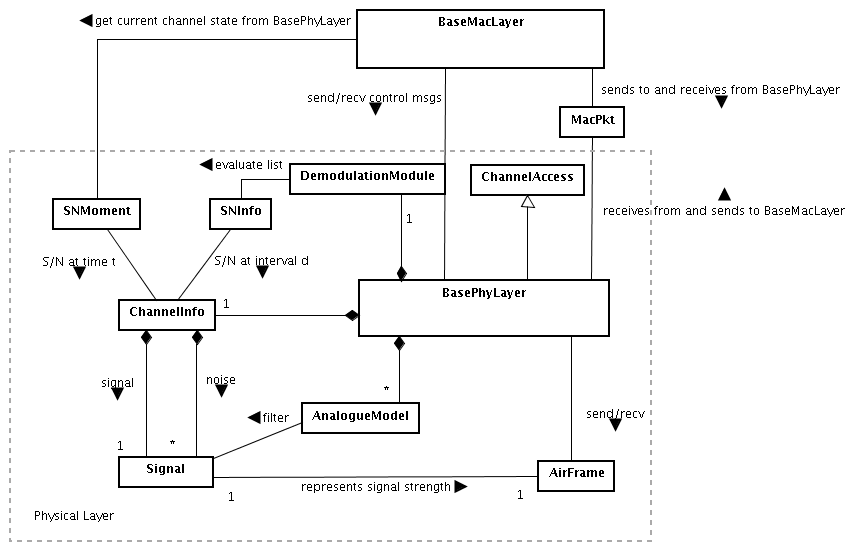
\includegraphics[width=400pt]{modelling/class_diagram.png}
 \caption{class graph}
 \label{fig: classgraph}
\end{figure}
\newpage

\subsection{The \h{\bp} interface}

In this section we focus on how one is able to communicate with the \h{\bp}, i.e. 
especially the \h{\bm} which is connected via an OMNeT-channel, OMNeT-controlchannel and holds a reference to \h{\bp}.
\h{\bm} can obtain information about the channelstate, i.e. idle (boolean) or RSSI by 
a simple method call. Further it is able to set current mode in \h{\bp} via method call.

\begin{figure}[H]
 \centering
 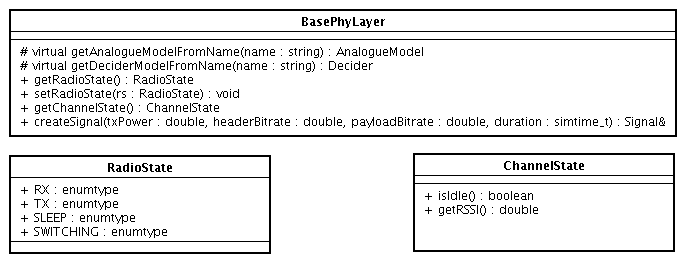
\includegraphics[width=340pt]{modelling/BasePhyLayer_members.png}
 \caption{BasePhyLayer interface}
 \label{fig: BasePhyLayer interface}
\end{figure}
\newpage


\subsection{AnalogueModel and Signal}


The Signal is designed one-dimensional (value-by-time) by default. The owner is able
to add and request values at a specific time point.
The Method getTimeIterator() return an appropriate SignalTimeIterator.
\begin{quote}
\emph{BEWARE: Anyone who subclasses Signal should make shure to have a properly
working SignalTimeIterator (subclassed) for it.}
\end{quote}

\begin{figure}[H]
 \centering
 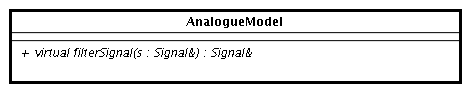
\includegraphics[width=340pt]{modelling/AnalogueModel_members.png}
 \caption{analogue model interface}
 \label{fig: analogue model interface}
\end{figure}

The AnalogueModel offers functionality to filter a referenced signal in a specified
interval and at a specific point in time. Therefore an appropriate SignalTimeIterator is needed!

\begin{figure}[H]
 \centering
 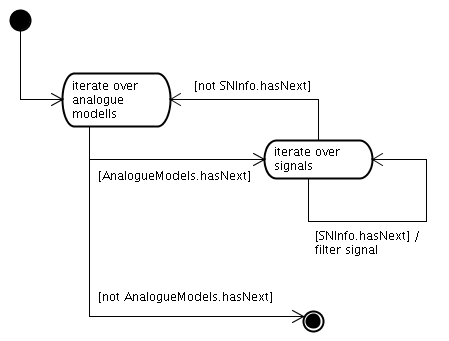
\includegraphics[width=300pt]{modelling/apply_analogue_modells_detail.png}
 \caption{application of analogue models}
 \label{fig: application analogue models}
\end{figure}
\newpage



\subsection{SNInfo and ChannelInfo}

ChannelInfo keeps track of all AirFrames on the channel. It does not differ between \textit{signal} and \textit{noise}. \h{\bp} is able to
add and remove references to certain AirFrames.
ChannelInfo is able to record the whole channel over time from a start to a stop signal and can return a vector of Signals (references) that intersect with a given time interval.\\
SNInfo is created by \h{\bp} when a packet arrives to collect all signals from the channel that intersect with the reception time interval of the packet.

\begin{figure}[H]
 \centering
 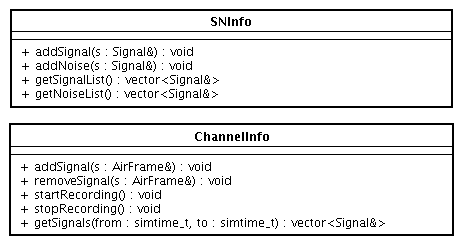
\includegraphics[width=340pt]{modelling/ChannelInfo_members.png}
 \caption{channel details}
 \label{fig: channel details}
\end{figure}

\newpage


\subsection{Decider}

The decider has two tasks:
\begin{enumerate}
	\item It decides whether we are able to receive a certain packet by evaluting
	the SNInfo for the packets preamble time interval, otherwise the packet will 	be considered noise
	\item When a packet has been received as a \textit{signal} the Decider 	returns a DeciderResult for that packet, that only contains correct/not correct 	by default.
\end{enumerate}


\begin{figure}[H]
 \centering
 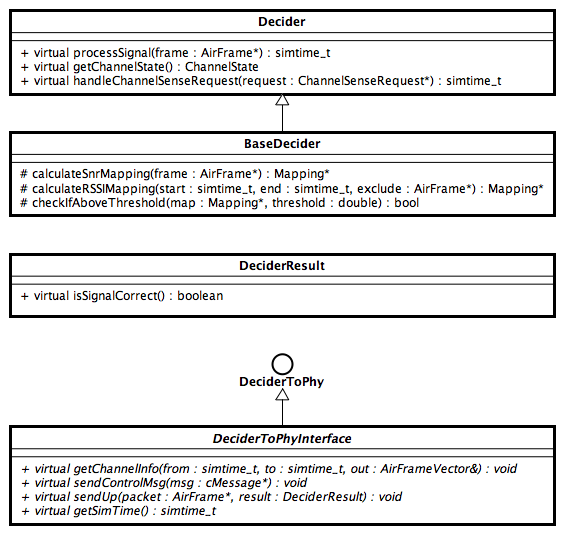
\includegraphics[width=340pt]{modelling/DeciderModule_members.png}
 \caption{Decider interface}
 \label{fig: Decider interface}
\end{figure}
\newpage

\subsection{AirFrame}


\begin{figure}[H]
 \centering
 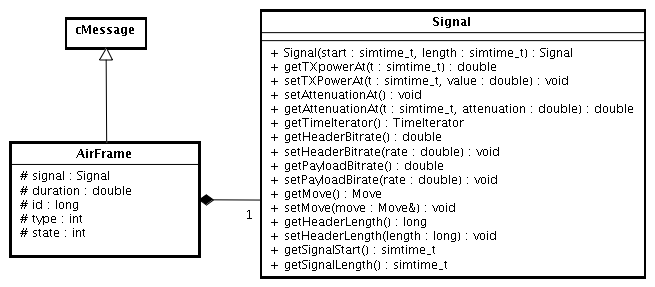
\includegraphics[width=300pt]{modelling/AirFrame_members.png}
 \caption{member arrangement in AirFrame and Signal}
 \label{fig: member AirFrame}
\end{figure}
\newpage


\subsection{Receiving and processing an AirFrame}

The reception of an AirFrame is divided into:
\begin{enumerate}
	
	\item optional propagation delay,
	\item reception of the preamble,
	\item application of AnalogueModels to the corresponding SNInfo,
	\item decision whether packet is considered noise (Decider),
	\item reception of the packet.
\end{enumerate}

Afterwards the packet is either dropped (if considered noise) or processed. 

\begin{figure}[H]
 \centering
 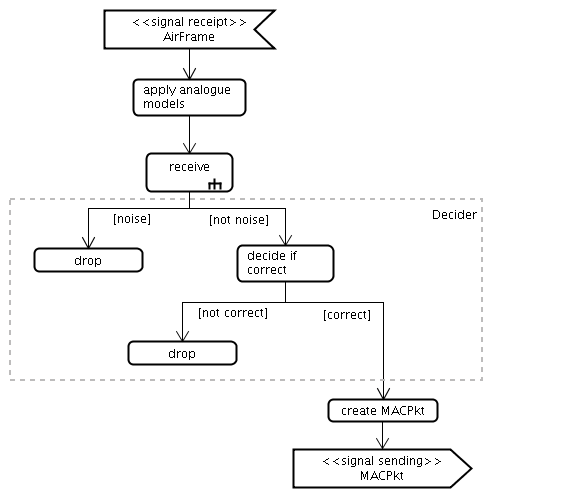
\includegraphics[width=340pt]{modelling/onAirFrame.png}
 \caption{receiving process}
 \label{fig: receiving process}
\end{figure}

\begin{figure}[H]
 \centering
 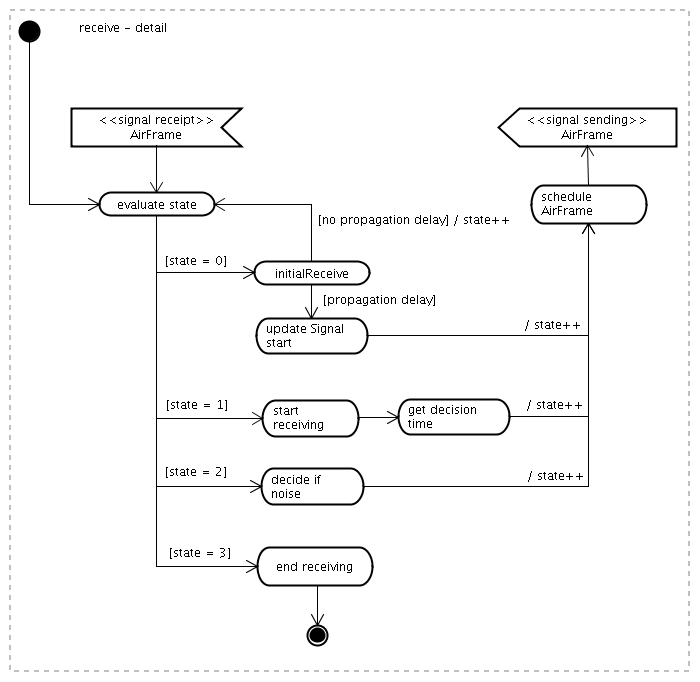
\includegraphics[width=340pt]{modelling/receive_detail.png}
 \caption{receive detail}
 \label{fig: receive detail}
\end{figure}

\begin{figure}[H]
 \centering
 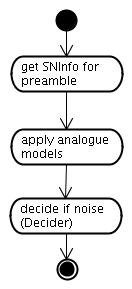
\includegraphics{modelling/end_preamble_detail.png}
 \caption{end preamble detail}
 \label{fig: end preamble detail}
\end{figure}

\newpage

\subsection{receiving a MacPkt}


\begin{figure}[H]
 \centering
 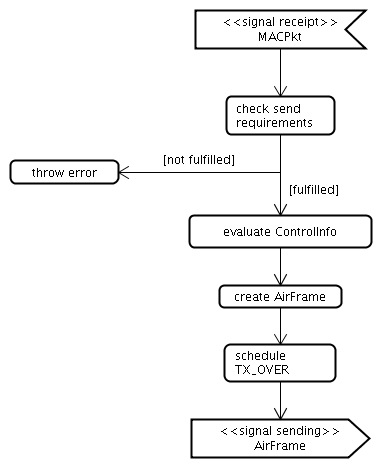
\includegraphics[width=300pt]{modelling/onMACPkt.png}
 \caption{sending process}
 \label{fig: sending process}
\end{figure}


%\subsection{provide status information to MAC}

%Passively provided information\req{provpassive}: \h{\bm} is equipped with a reference to \h{\bp} in order to obtain information
%about channelstate\req{channelstate} and current mode\req{currentmode} by
%simple method calls. \\
%Actively provided information\req{provactive}: A cMessage of the kind TX\_OVER
%is sent to MAC-Layer when a sending transmission is over\req{txover}, \saf{sending process}.

%\subsection{switch states}

%Furthermore the MAC-Layer is able to set the current mode (RX, TX, SLEEP)\req{switchmode} of the Phy-Layer by a simple method call.
%\h{\bp} will change to switching state and schedule itself the appropriate timer for the switching interval\req{switchtimes}, \saf{mode state machine}.


%\subsection{send packets}

%Since \h{\bm} has a reference to \h{\bp} it can obtain information about the mode the radio is is currently in\req{sendPreqMode}, it is not already sending to the channel on its own\req{sendPreqSending} and the channel is idle\req{sendPreqIdle} via method calls, \saf{BasePhyLayer interface}.

%The class MacToPhyControlInfo is designed as the container for control info\req{packetFromMac} the MAC-Layer
%wants to attach to the packet given down to Phy-Layer for sending.
%The packet itself is handed down as a MacPkt via OMNeT-channel. 

%\begin{figure}[h]
% \centering
% 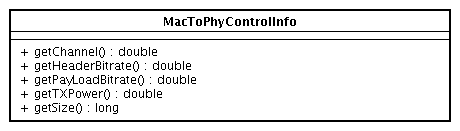
\includegraphics[width=340pt]{modelling/MacToPhyCtrlInfo_members.png}
% \caption{MacToPhyControlInfo interface}
% \label{fig: MacToPhyCtrlInfo interface}
%\end{figure}













